\documentclass[12pt]{article}
\usepackage{setspace}
\setlength{\parindent}{4em}
\usepackage{fancyvrb}
\usepackage{graphicx}
\usepackage{geometry}
\renewcommand\thesection{\arabic{section}}
\renewcommand\thesubsection{\thesection.\arabic{subsection}}
\geometry{letterpaper, portrait, margin=1in}

%%%Title Page%%%
\title{\vspace{3cm}Lab 06\bigbreak Adding Memory and Bootstrapping Circuit}
\author{
{\normalsize
\begin{tabular}{l r r}
 & \textbf{Ryan Cruz} & \textbf{Zachary Davis}\\
\textbf{Category} & ryan.cruz25@uga.edu & zachdav@uga.edu\\
\hline
Pre-lab 						  & 40 & 60\\
In-lab Module \& Testbench Design & 50 & 50\\
In-lab Testbench Sim. \& Analysis & 50 & 50\\
In-lab FPGA Synthesis \& Analysis & 50 & 50\\
Lab Report Writing 				  & 60 & 40\\
\end{tabular}
}}
%%%%%%%%%%%%%%%%%

\begin{document}
\maketitle
\newpage
\setstretch{2.5} % for custom spacing
\tableofcontents
\setstretch{1} % for custom spacing
\newpage

\section{Lab Purpose} \vspace{-.7cm} \line(1,0){470}
	\paragraph{}
		Entering this lab, we now have the Toy Processor complete with the ability to run simple programs that do not need memory. As the next logical step, we will add Random Access Memory and Read Only Memory for the processor. With this added, we can finally but this on the FPGA board and load any simple program.
		
\section{Implementation Details} \vspace{-.7cm} \line(1,0){470}
		\subsection{Prelab}
			\hfill

		\begin{figure}[h]
		\centering
			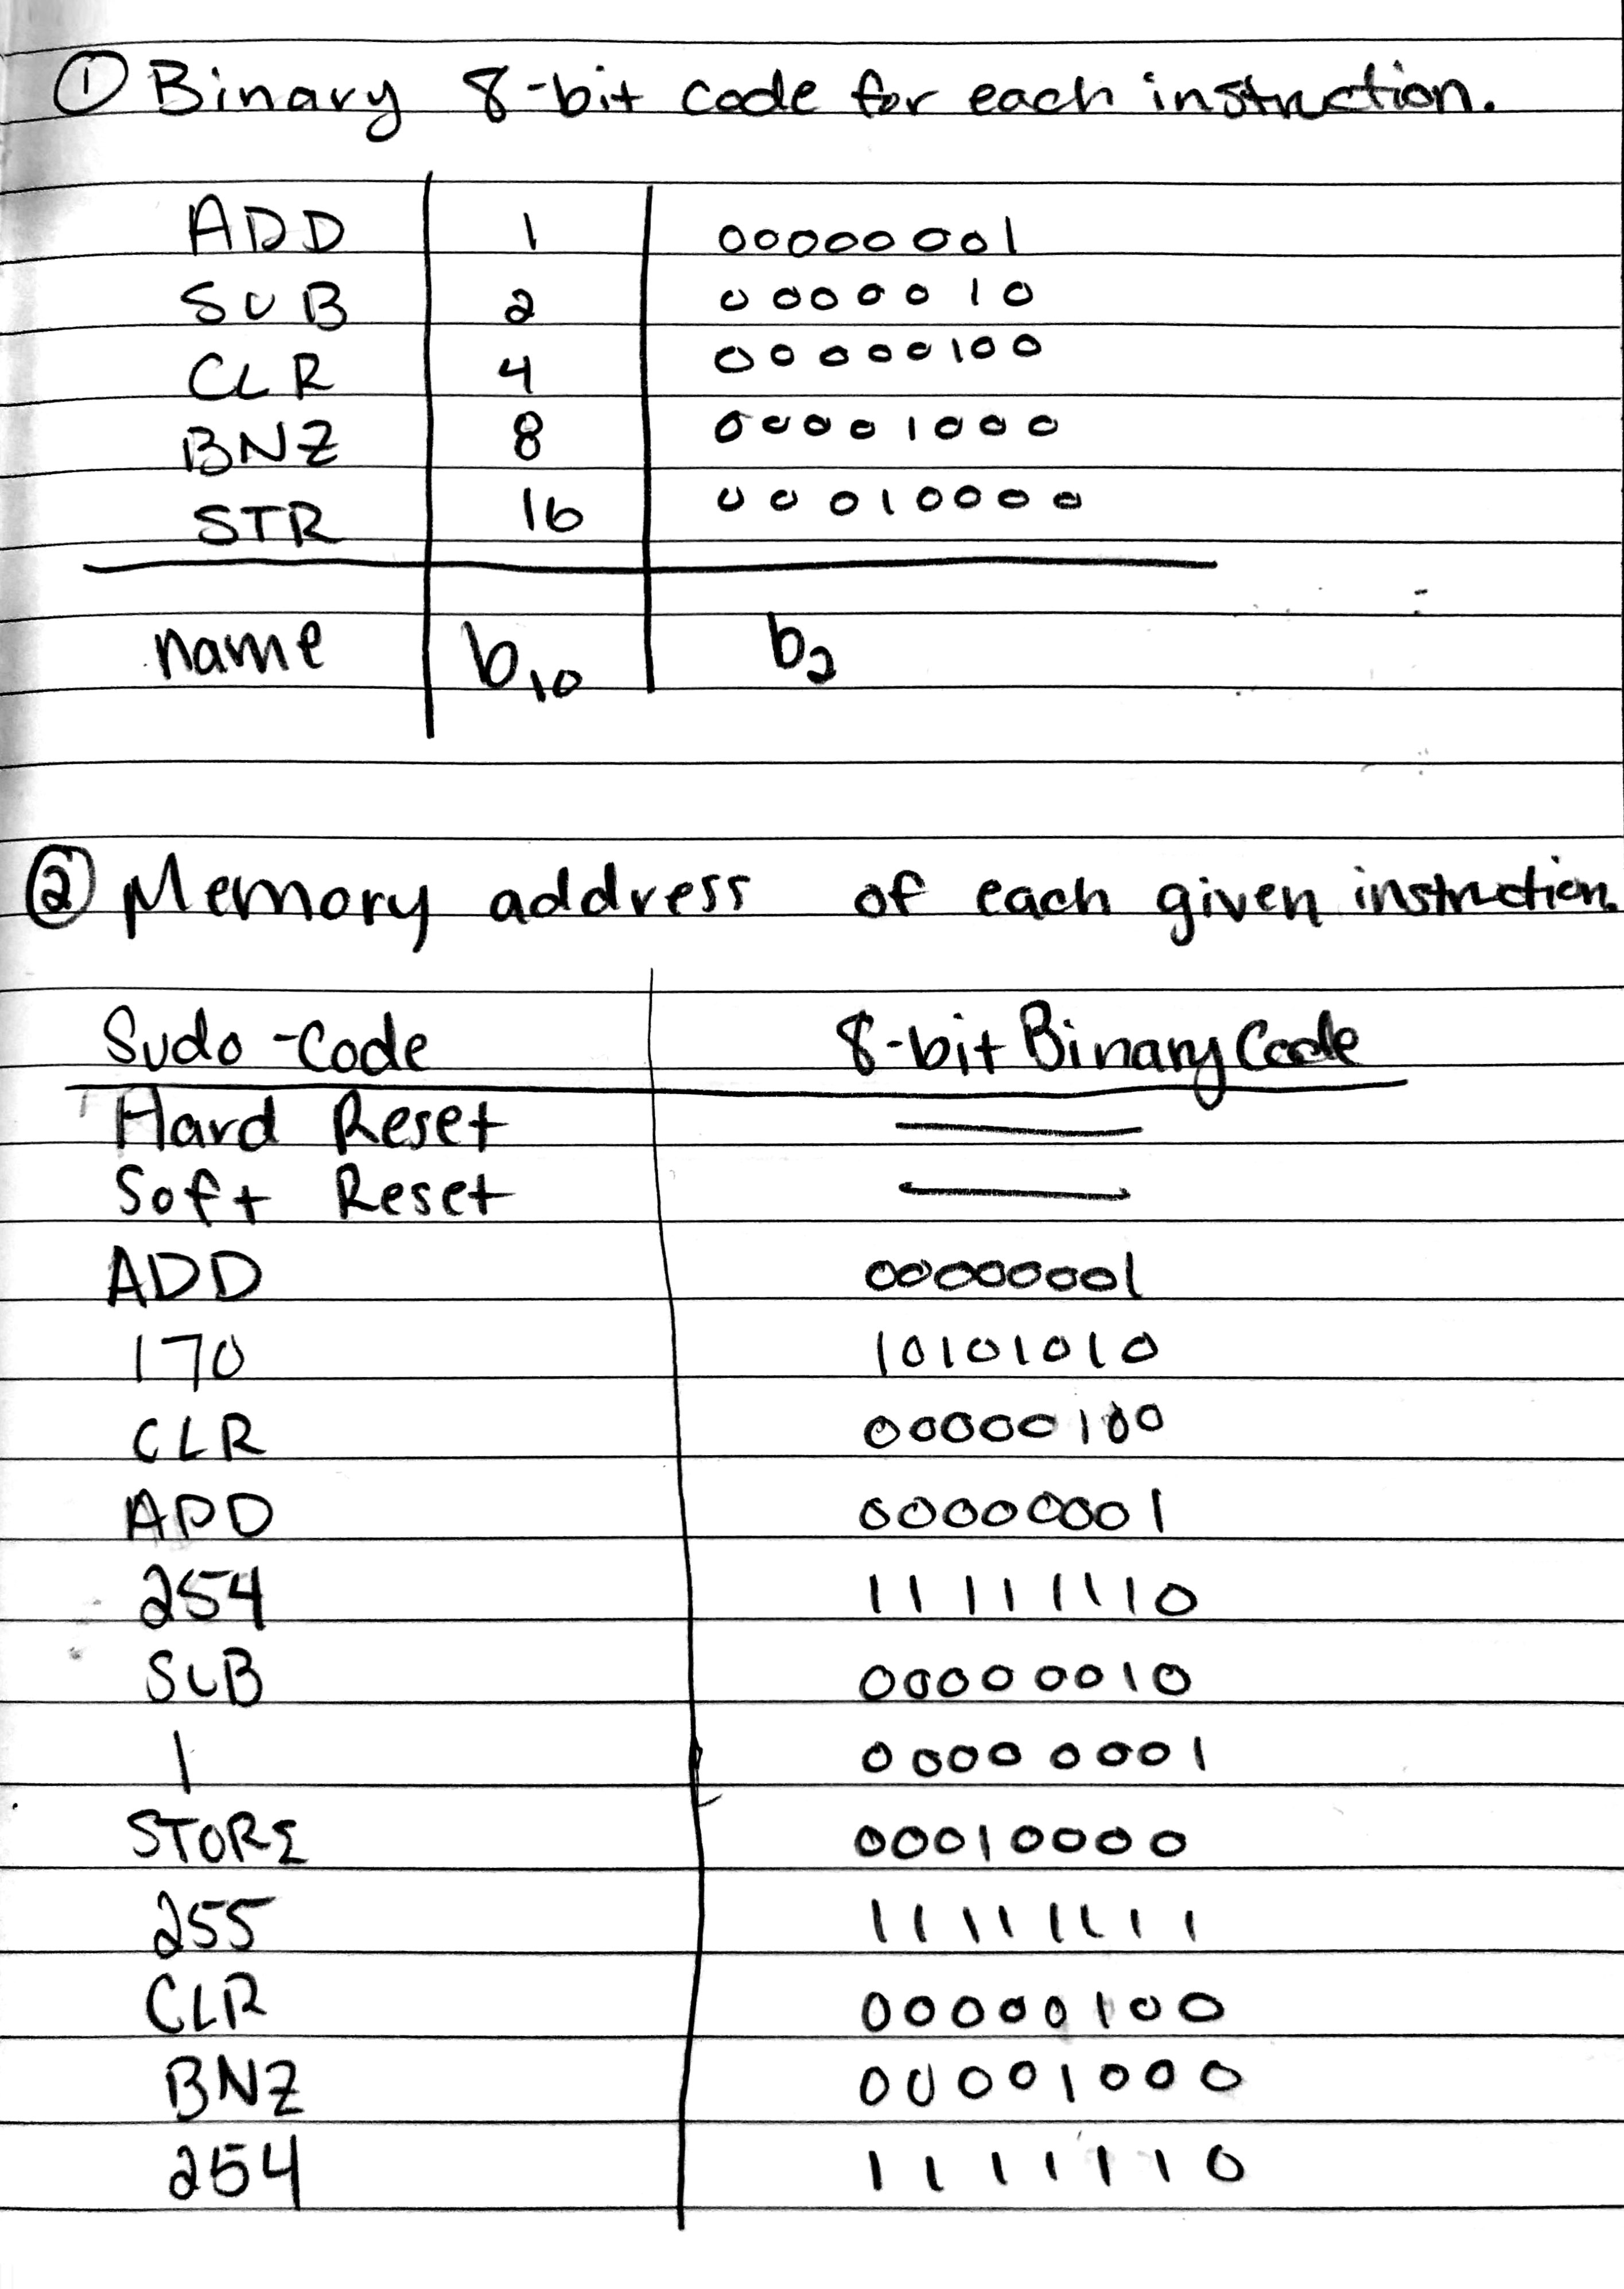
\includegraphics[scale=.7]{Prelab.pdf}
			\caption{Memory Bootstrapping circuit to copy the entire contents of the ROM array into the RAM array.}
		\end{figure}
			
		\begin{figure}[h]
			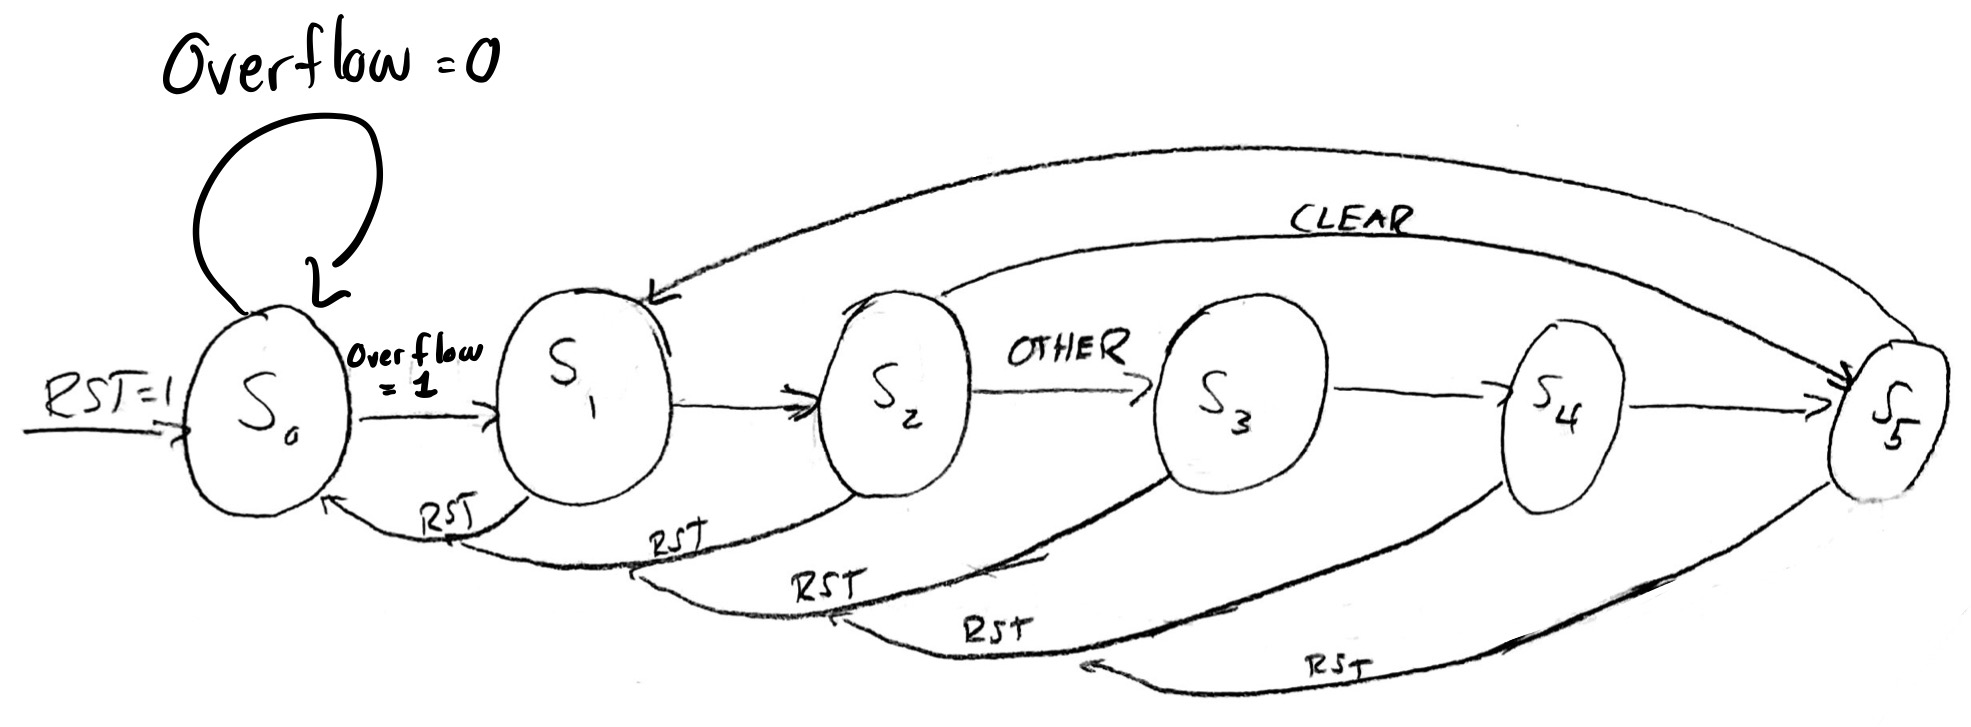
\includegraphics[scale=.175]{Prelab2}
			\caption{Modification of the controller so that we do not transition from S0 to S1 before the memory bootstrapping is complete.}
		\end{figure}
		
		\newpage
	\subsection{Part 1 - Include ROM}
	The ROM array was given to us as a schematic of ROM32X1 modules. Below is a testbench to make sure it is operating correctly. We also initialized the first row of modules with the following values:

\begin{flushleft}
\begin{tabular}{|l|}
\hline
00000912 \\
00000910 \\
00000912 \\
00000990 \\
00000D12 \\
00000B14 \\
00000932 \\
00000149 \\
\hline
\end{tabular}
\end{flushleft}

		
		\begin{Verbatim}[frame=single, fontsize= \small]
//ROM Testbench
`timescale 1ns / 1ps

module ROM_array_ROM_array_sch_tb();

// Inputs
   reg [7:0] ADDR = 8'b00000000;

// Output
   wire [7:0] DATA_OUT;

// Bidirs

// Instantiate the UUT
   ROM_array UUT (
		.ADDR(ADDR), 
		.DATA_OUT(DATA_OUT)
   );
// Initialize Inputs
       initial begin
			#400;
			ADDR = 8'b00100000;
			#100;
			ADDR = 8'b00000001;
			end
endmodule
		\end{Verbatim}
		The test bench simply executes one address change to show that it is working properly. Refer to the Expiremental Results section to view the wavefrom results of this testbench.
		\begin{center}
			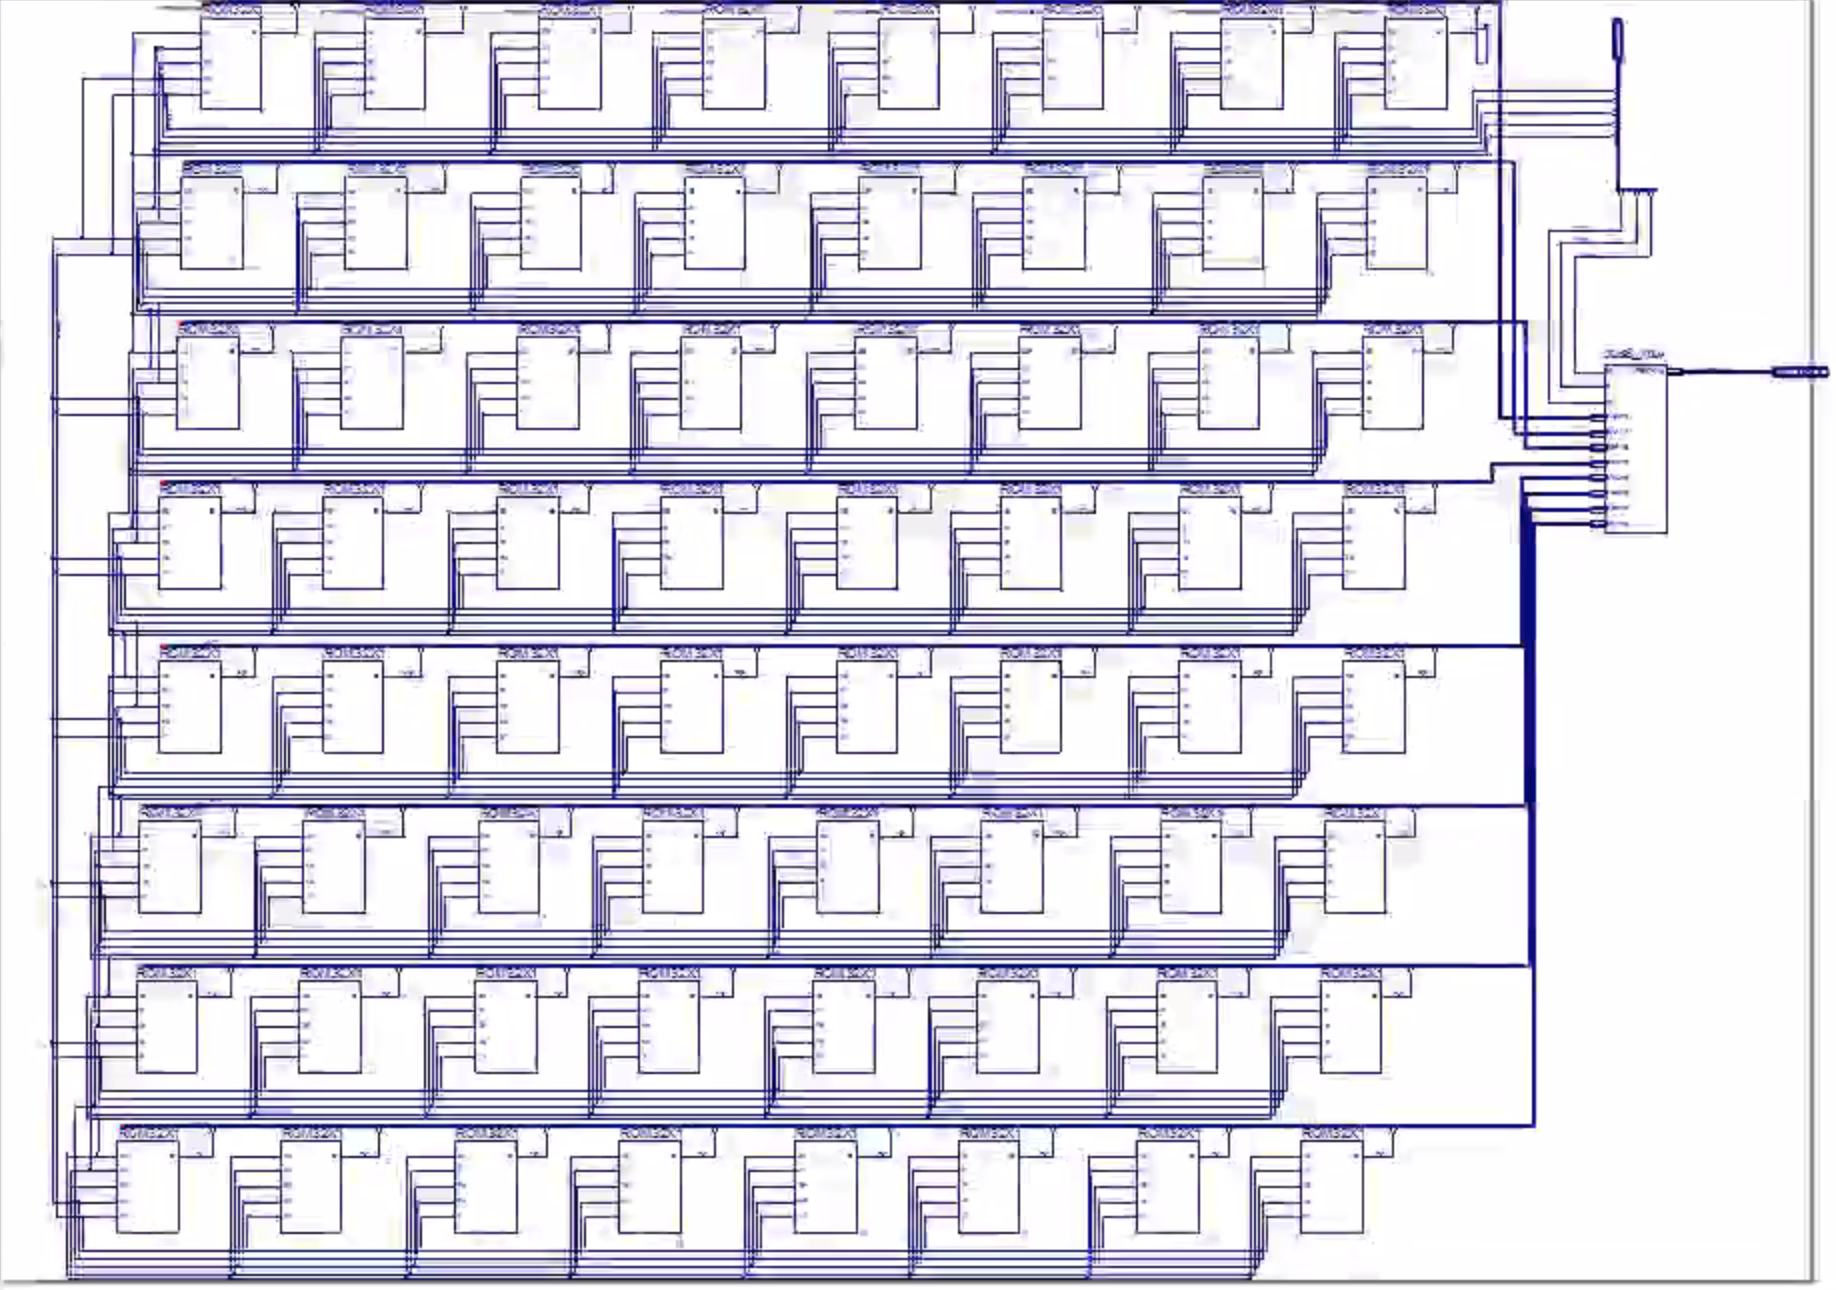
\includegraphics[scale=.5]{ROM.PNG}
		\end{center}

		\newpage
		\subsection{Part 2 - RAM}
		The ROM array was given to us as a schematic as well. Below is a testbench to make sure it is operating correctly.

		\begin{Verbatim}[frame=single, fontsize= \small]
//RAM_array_tb.v
`timescale 1ns/1ps
module RAM_array_tb;

reg [7:0] ADDR = 8'b00000000;
reg CLK = 1'b0;
reg [7:0] DATA_IN = 8'b00000000;
reg WE = 1'b0;
wire [0:7] DATA_OUT1;

initial // Clock process for CLK
begin
	forever 
		begin
			CLK = 1'b0;
			#100;
			CLK = 1'b1; 
			#100;
		end
	end
RAM_array UUT (
.ADDR(ADDR),CLK(CLK),.DATA_IN(DATA_IN),.WE(WE),.DATA_OUT1(DATA_OUT1));

initial begin
#85;
DATA_IN = 8'b11111111;
#200;
WE = 1'b1;
ADDR = 8'b00010000;
#600;
WE = 1'b0;
#200;
ADDR = 8'b00100000;
#600;
ADDR = 8'b00010000;

end
endmodule
		\end{Verbatim}
		This test bench is similar to the ROM one in purpose, simply executing a write to make sure it works. Refer to the Expiremental Results section to view the wavefrom results of this testbench.
		\begin{center}
 		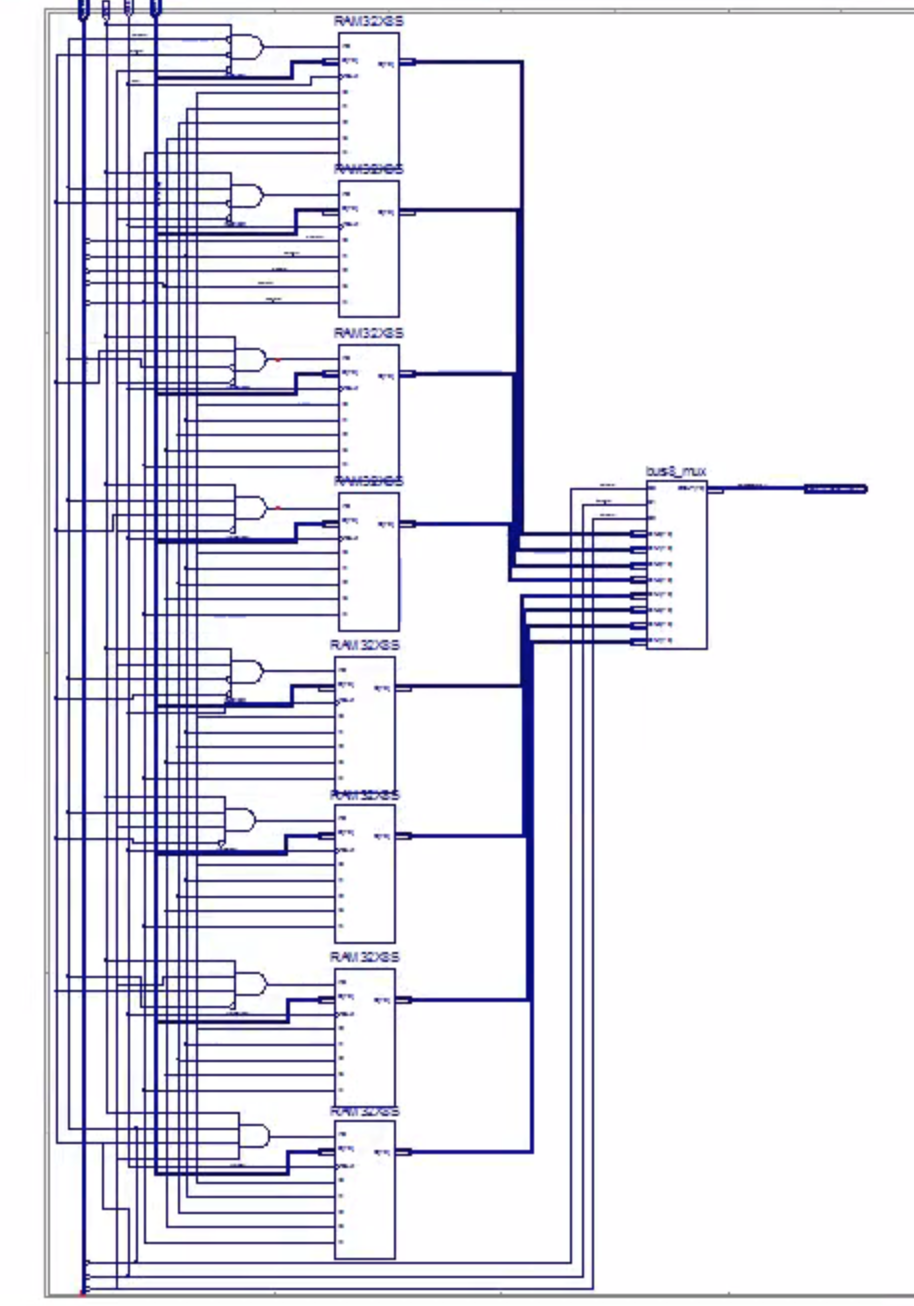
\includegraphics[scale=0.4]{RAM.png}\\
 	\end{center}

		\subsection{Part 3 - Memory Bootstrapping}
		The design was shown in the prelab, and below is the final schematic we made.

		\begin{figure}[h]
			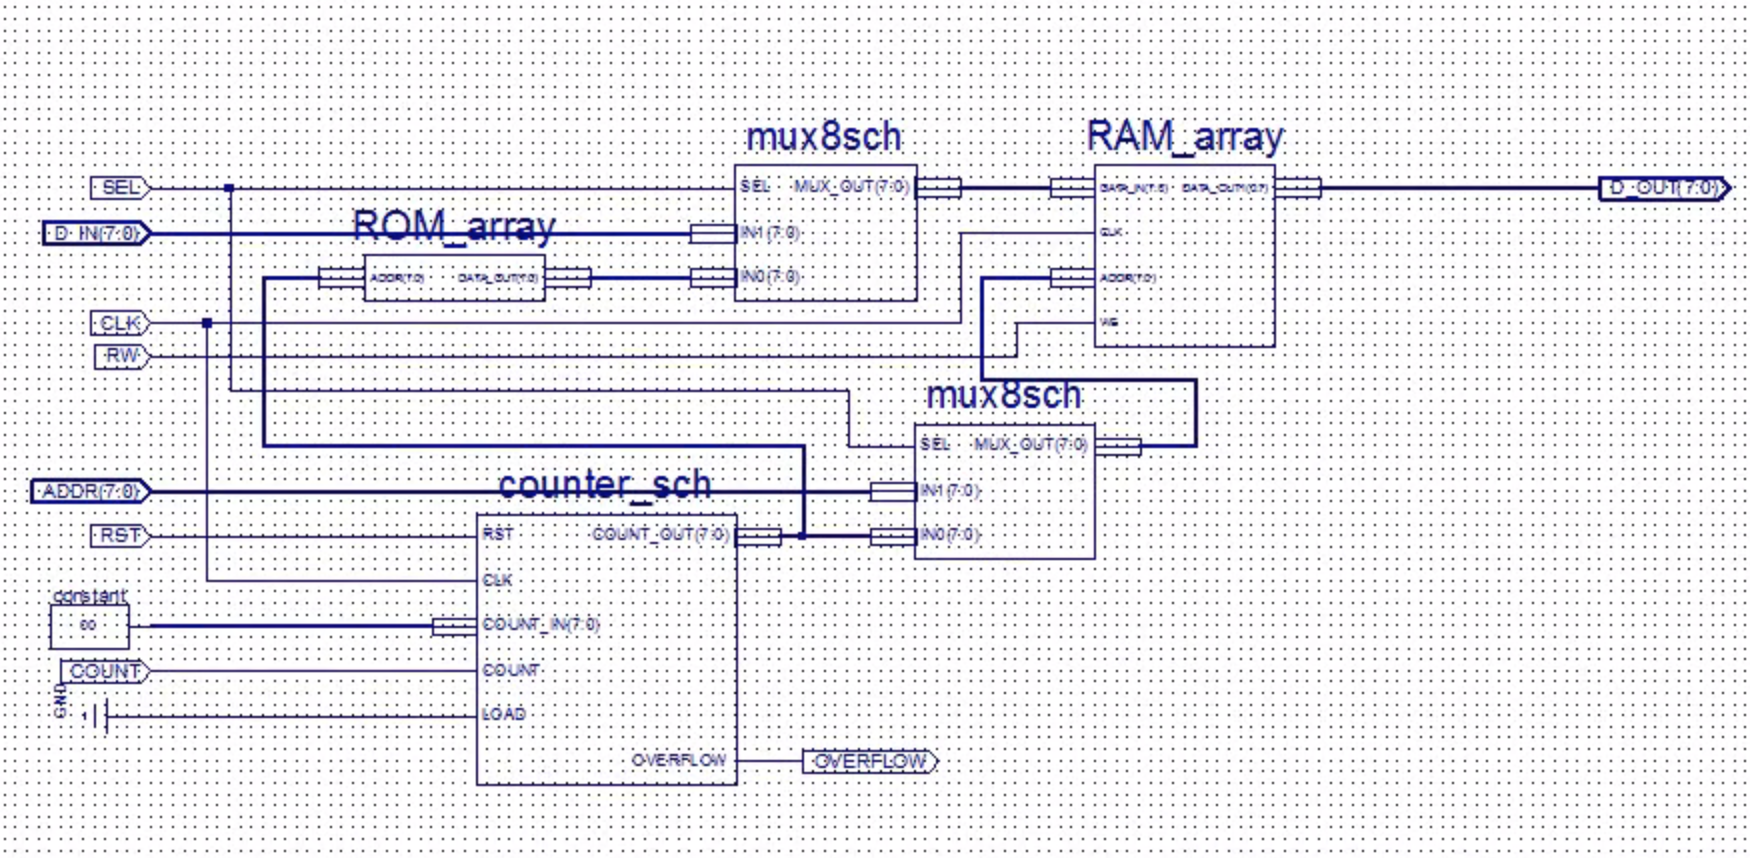
\includegraphics[scale=.5]{mem.png}
			\caption{Memory Bootstrapping Schematic.}
		\end{figure}



		\subsection{Part 4 - Integration}

		\begin{figure}[h]
			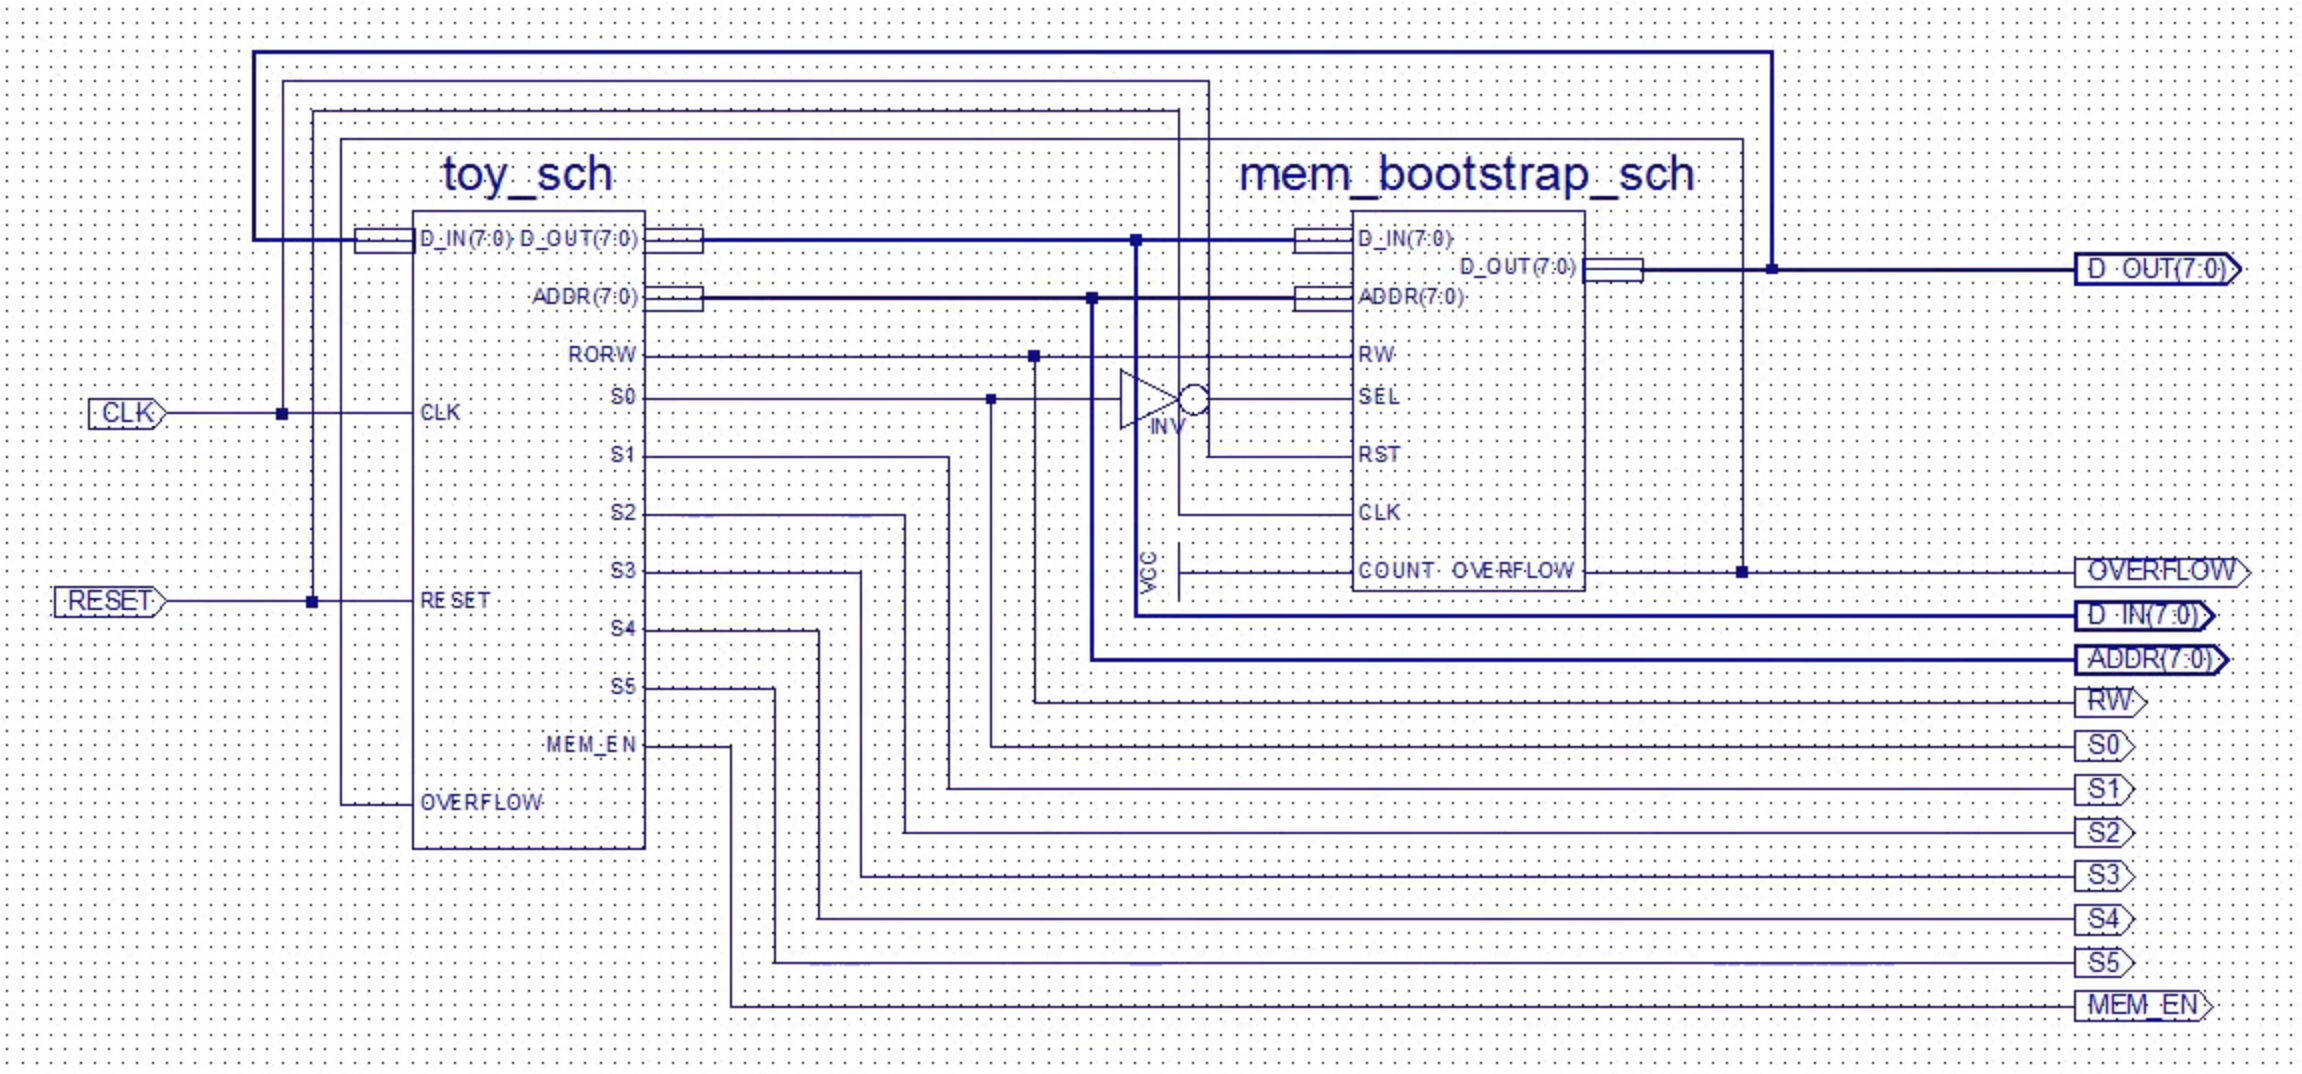
\includegraphics[scale=.4]{toy.png}
			\caption{Toy Processor Overall Schematic.}
		\end{figure}

		\begin{Verbatim}[frame=single, fontsize= \small]
`timescale 1ns / 1ps

module toyProcessor_overall_toyProcessor_overall_sch_tb();

// Inputs
   reg CLK;
   reg RESET;

// Output
	wire [7:0] D_IN;
   wire [7:0] D_OUT;
   wire [7:0] ADDR;
   wire RW;
	wire S0;
   wire S1;
   wire S2;
   wire S3;
   wire S4;
   wire S5;
   wire MEM_EN;
   wire OVERFLOW;

// Instantiate the UUT
   toyProcessor_overall UUT (
		.D_OUT(D_OUT), 
		.CLK(CLK), 
		.RESET(RESET), 
		.ADDR(ADDR), 
		.RW(RW), 
		.S1(S1), 
		.S2(S2), 
		.S3(S3), 
		.S4(S4), 
		.S5(S5), 
		.MEM_EN(MEM_EN), 
		.D_IN(D_IN), 
		.S0(S0), 
		.OVERFLOW(OVERFLOW)
   );
// Initialize Inputs
	initial
		begin forever
			begin
				CLK = 1'b0;
				#50;
				CLK = 1'b1;
				#50;
			end
		end
		
	initial
		begin
			RESET = 1;
			#300
			RESET = 0;
		end
endmodule
		\end{Verbatim}


\newpage			
\section{Experimental Results}\vspace{-.7cm} \line(1,0){470}

\begin{center}
	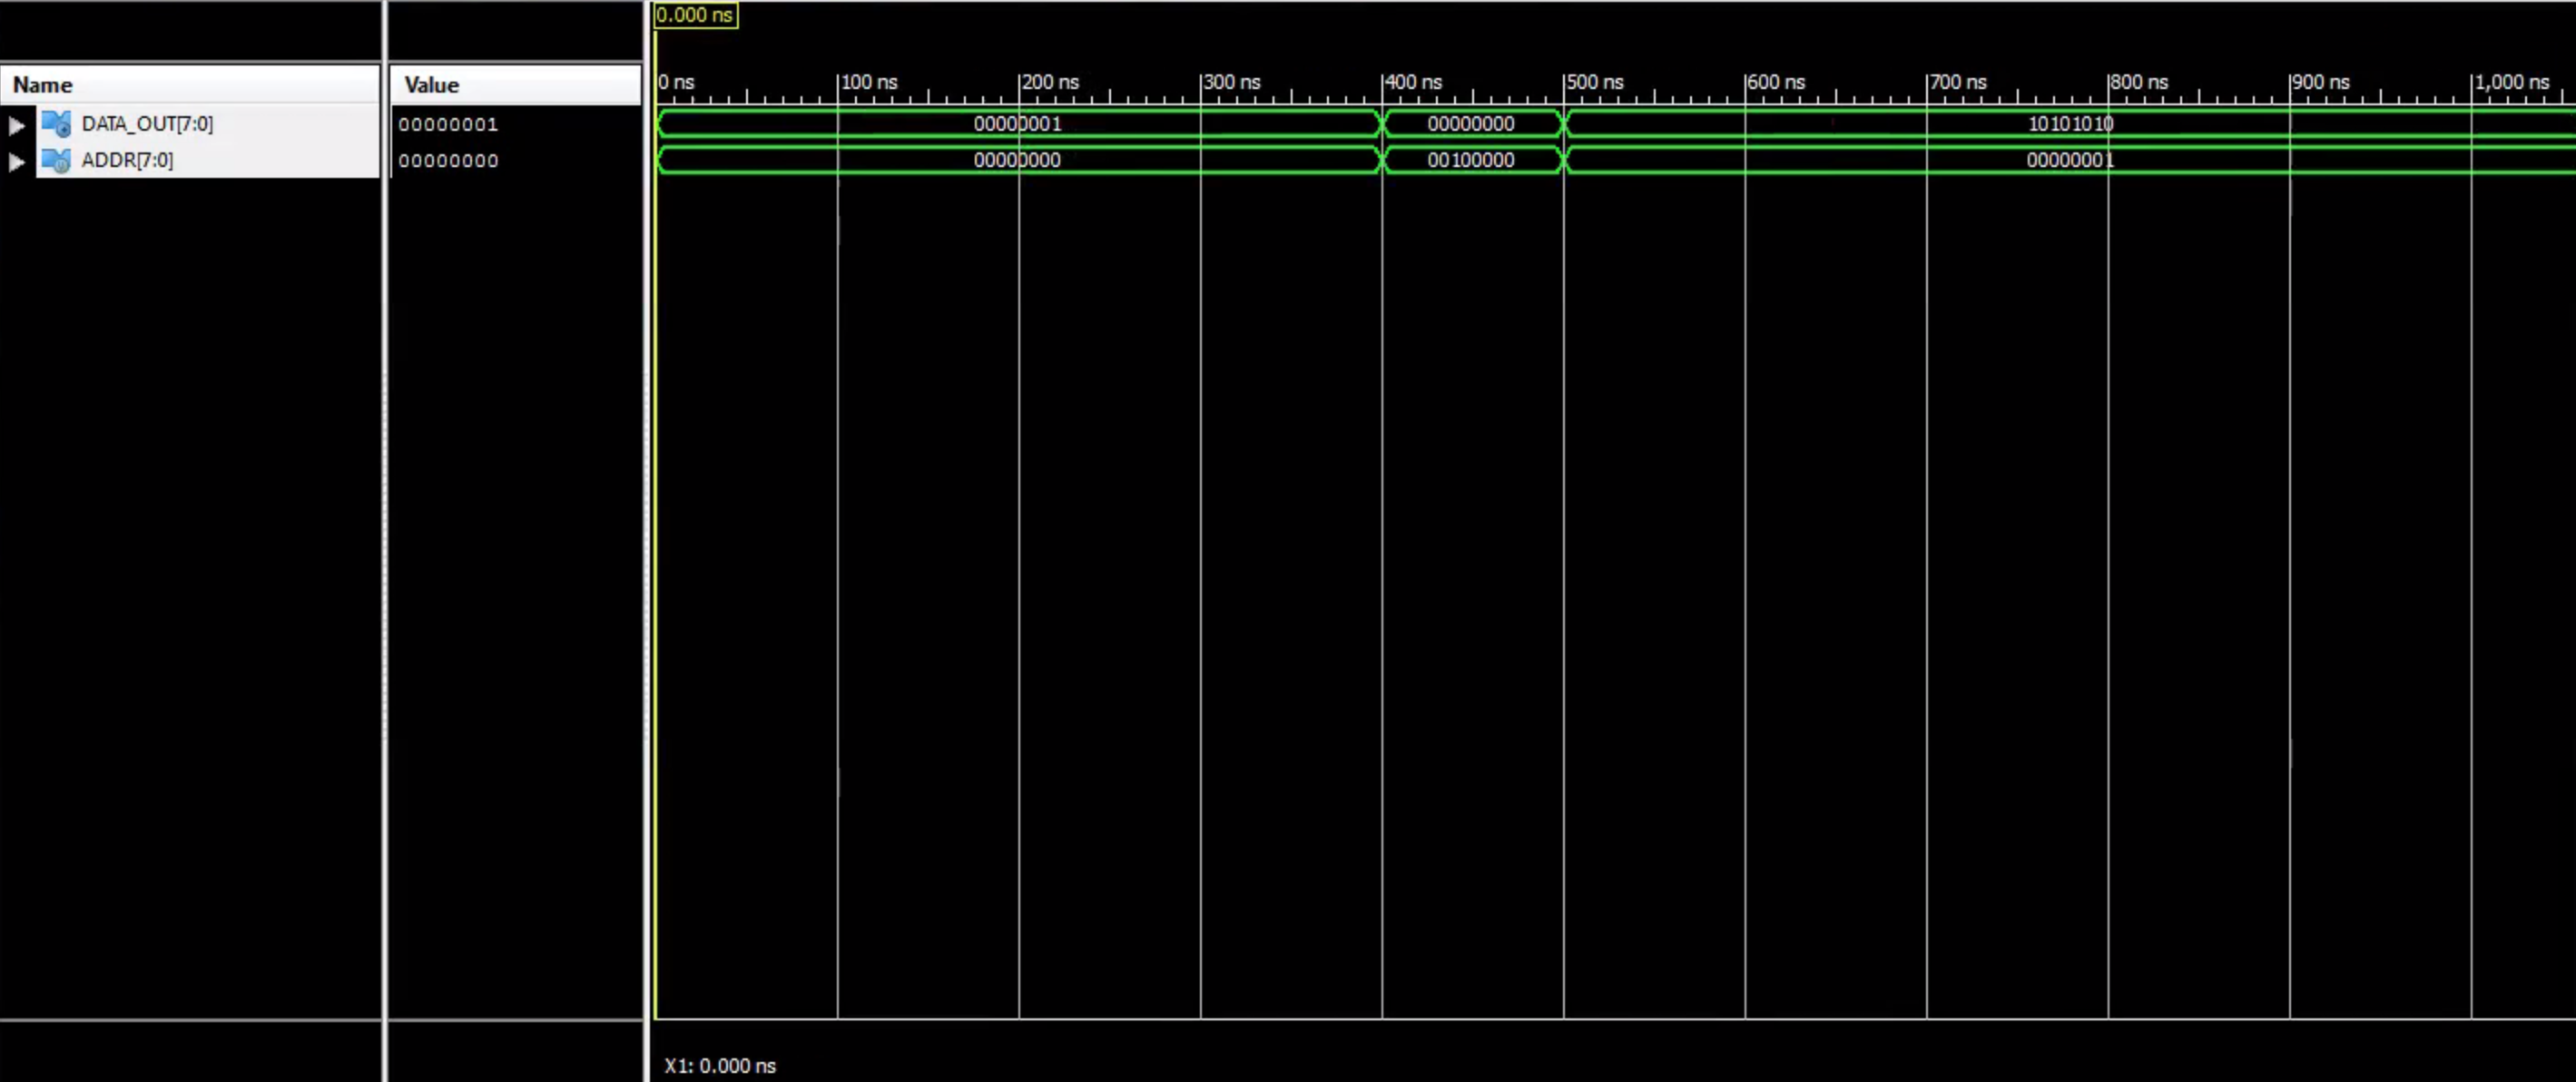
\includegraphics[scale=.3]{ROM_tb.png}\\
	This is our ROM testbench and using the chart above in the ROM section you can match the addresses with the output given.\\
	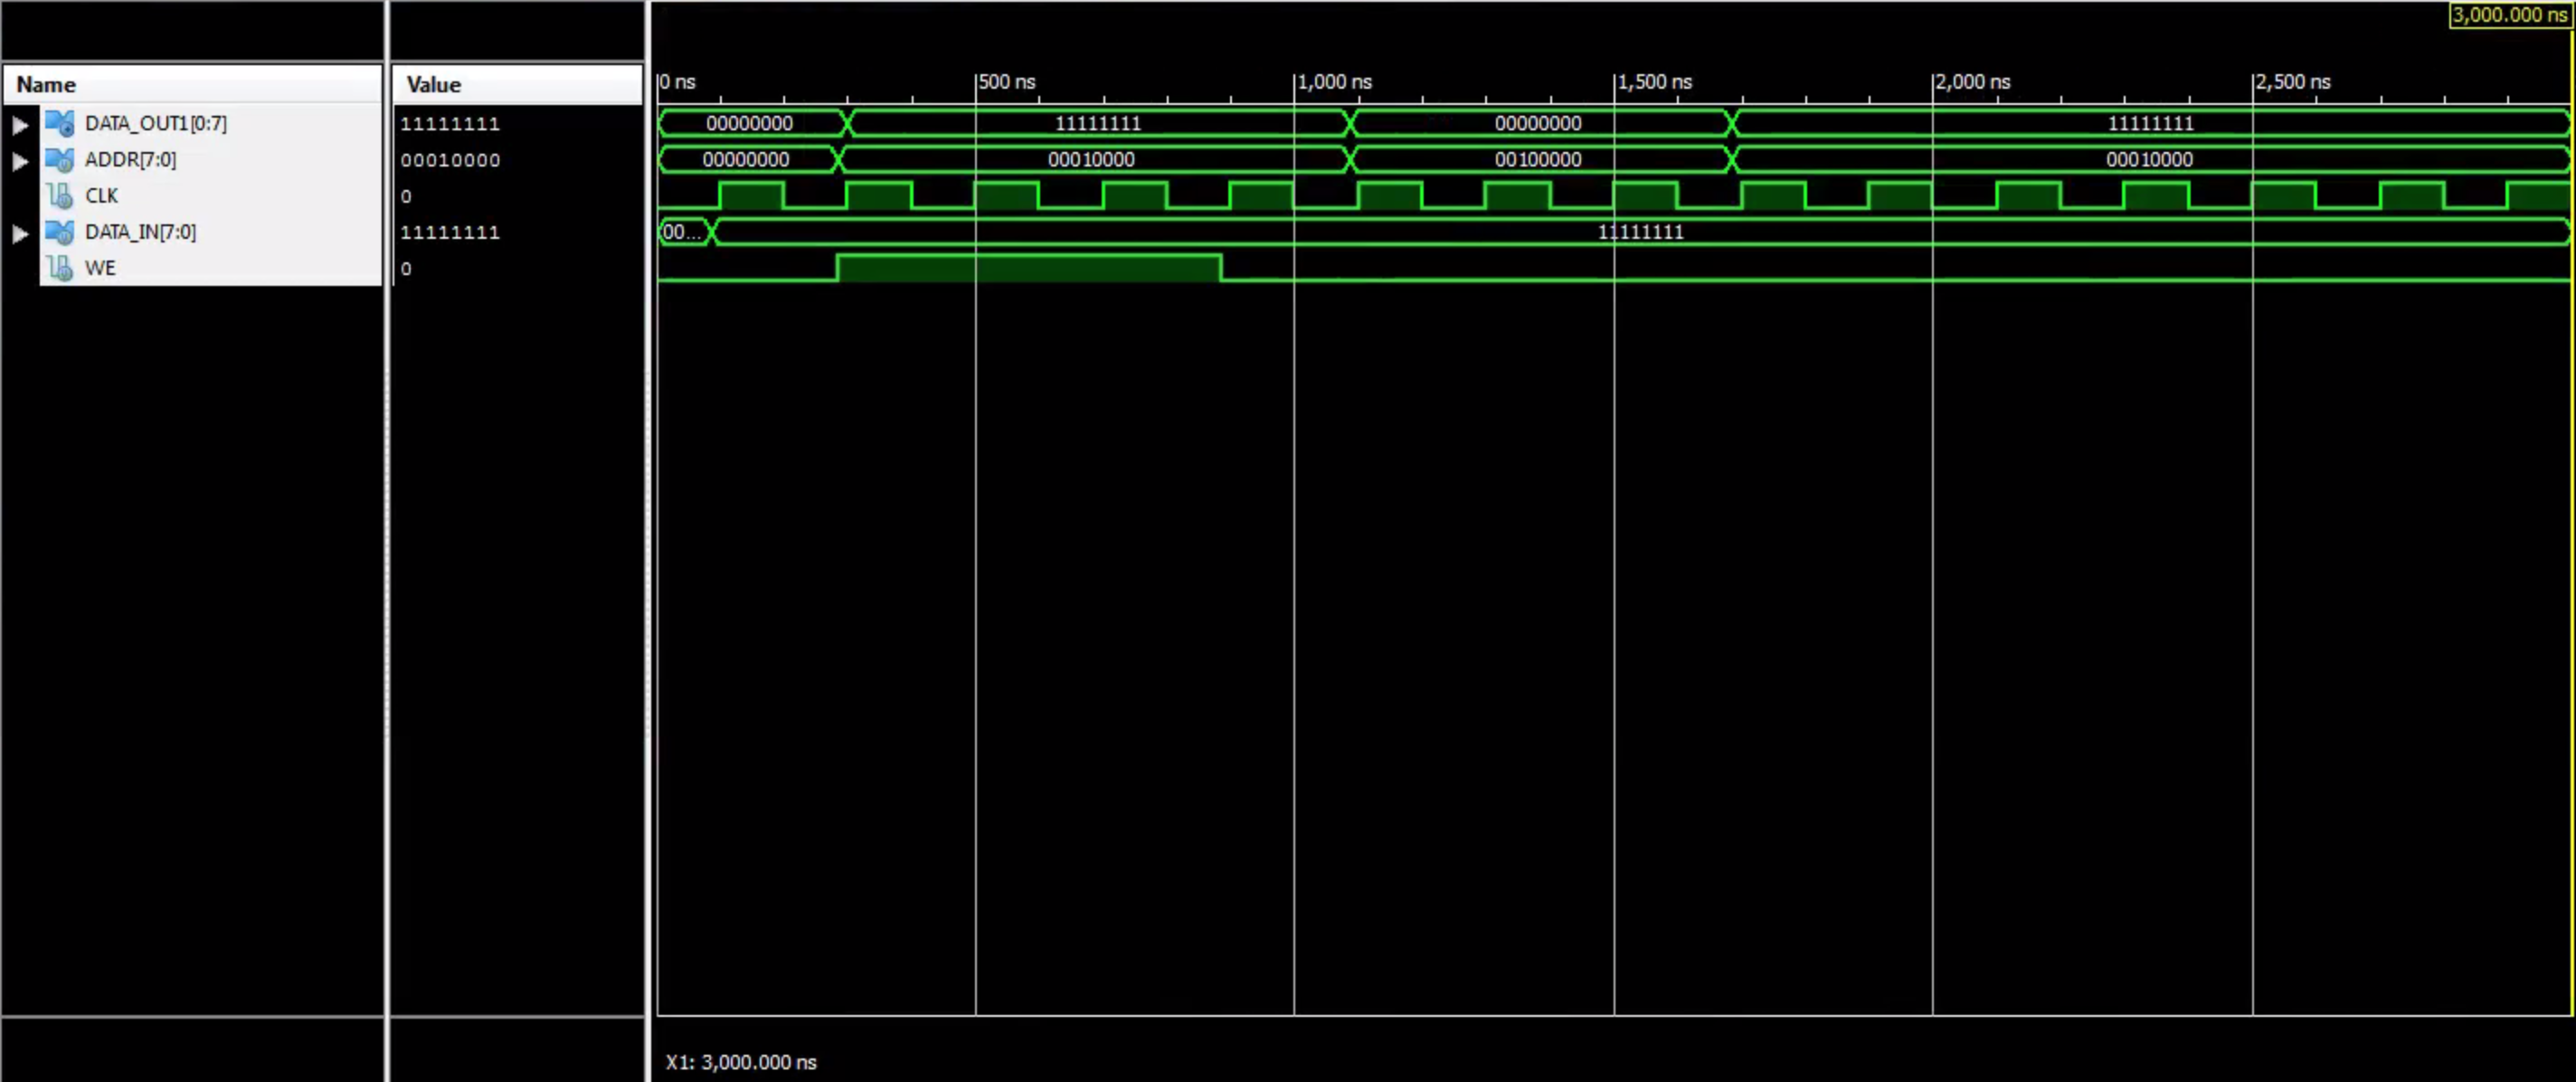
\includegraphics[scale=.3]{RAM_tb.png}\\
	This is out RAM testbench and you can again see and verify what is stored in the tested address as well as se us write something to RAM. It is worth noting that nothing is actually written until WE goes high.\\
	\newpage
	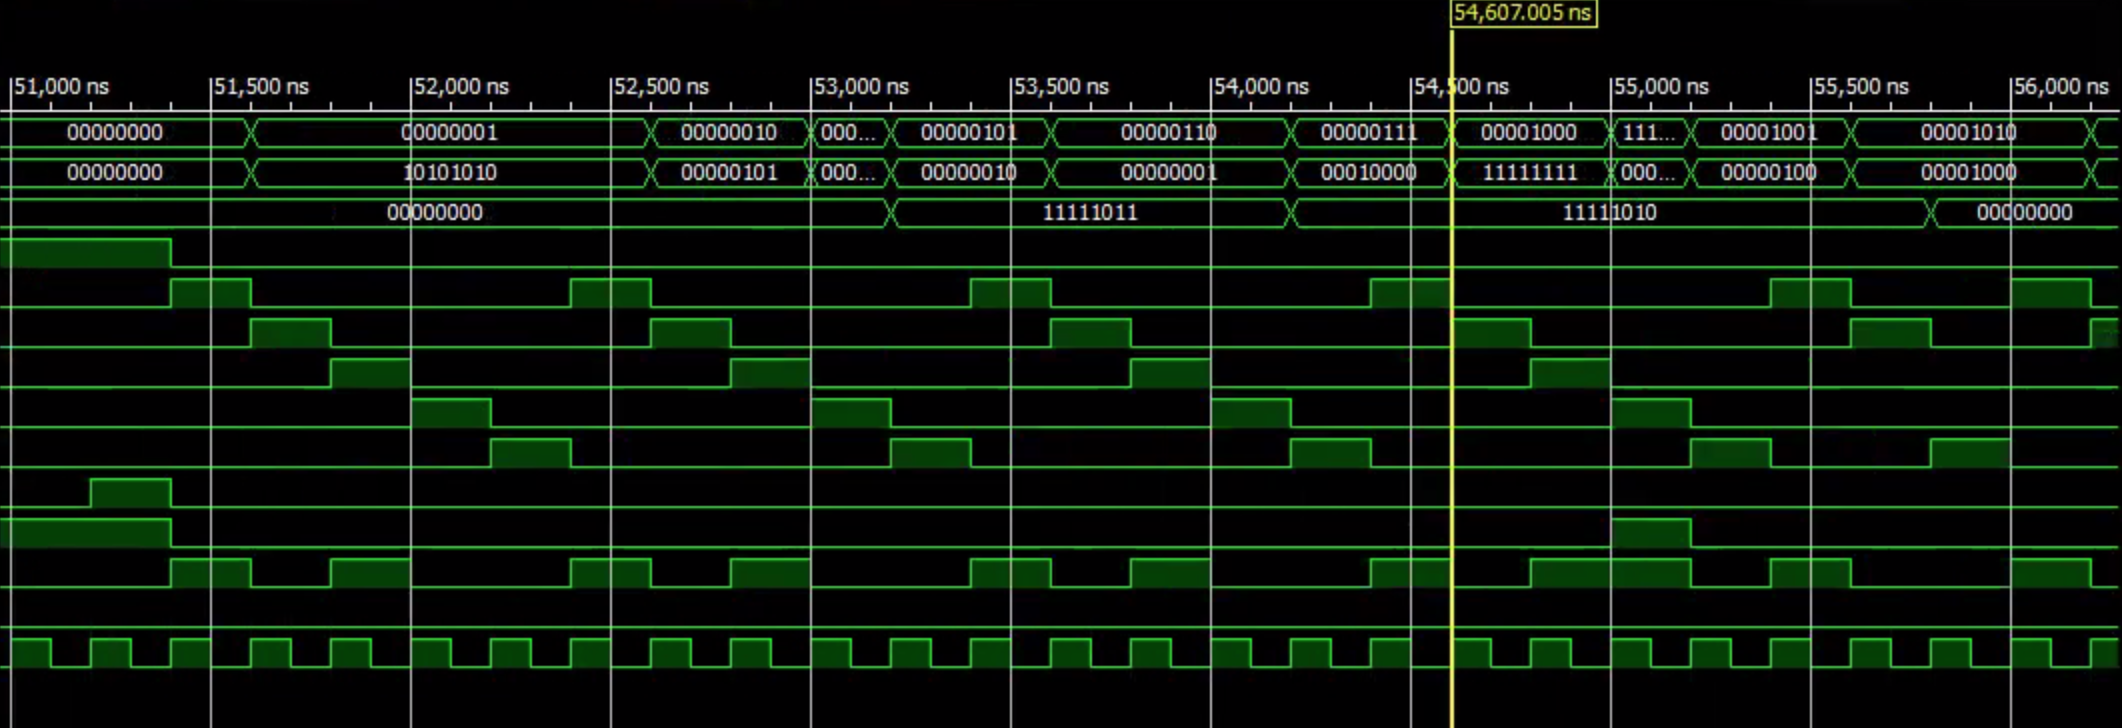
\includegraphics[scale=.4]{tb1.png}
	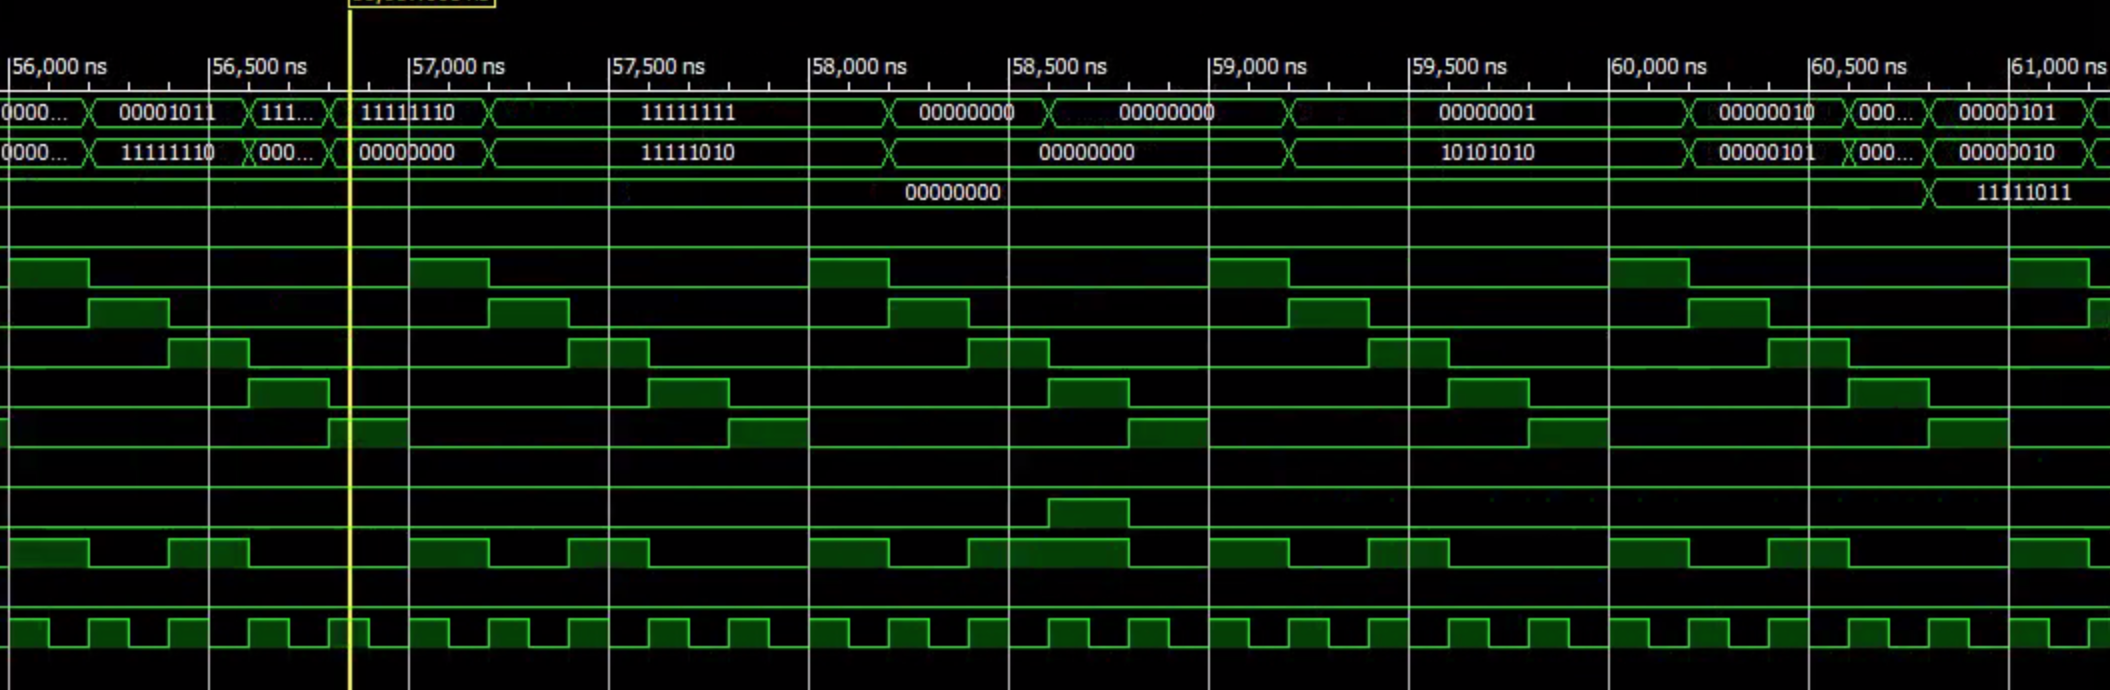
\includegraphics[scale=.4]{tb2.png}
	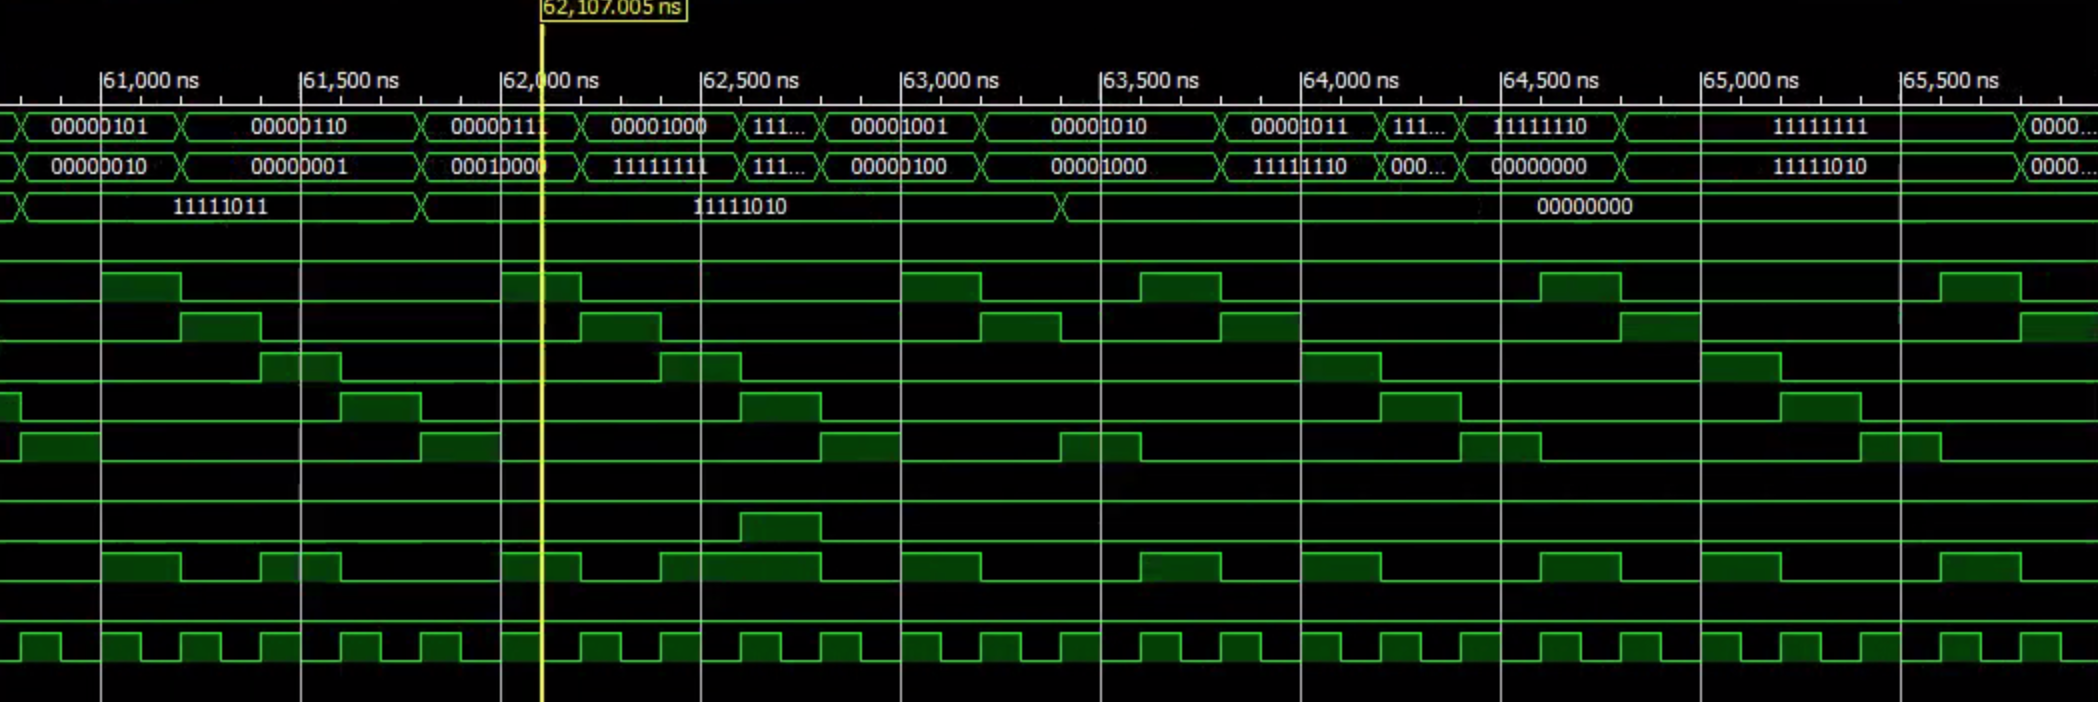
\includegraphics[scale=.4]{tb3.png}
	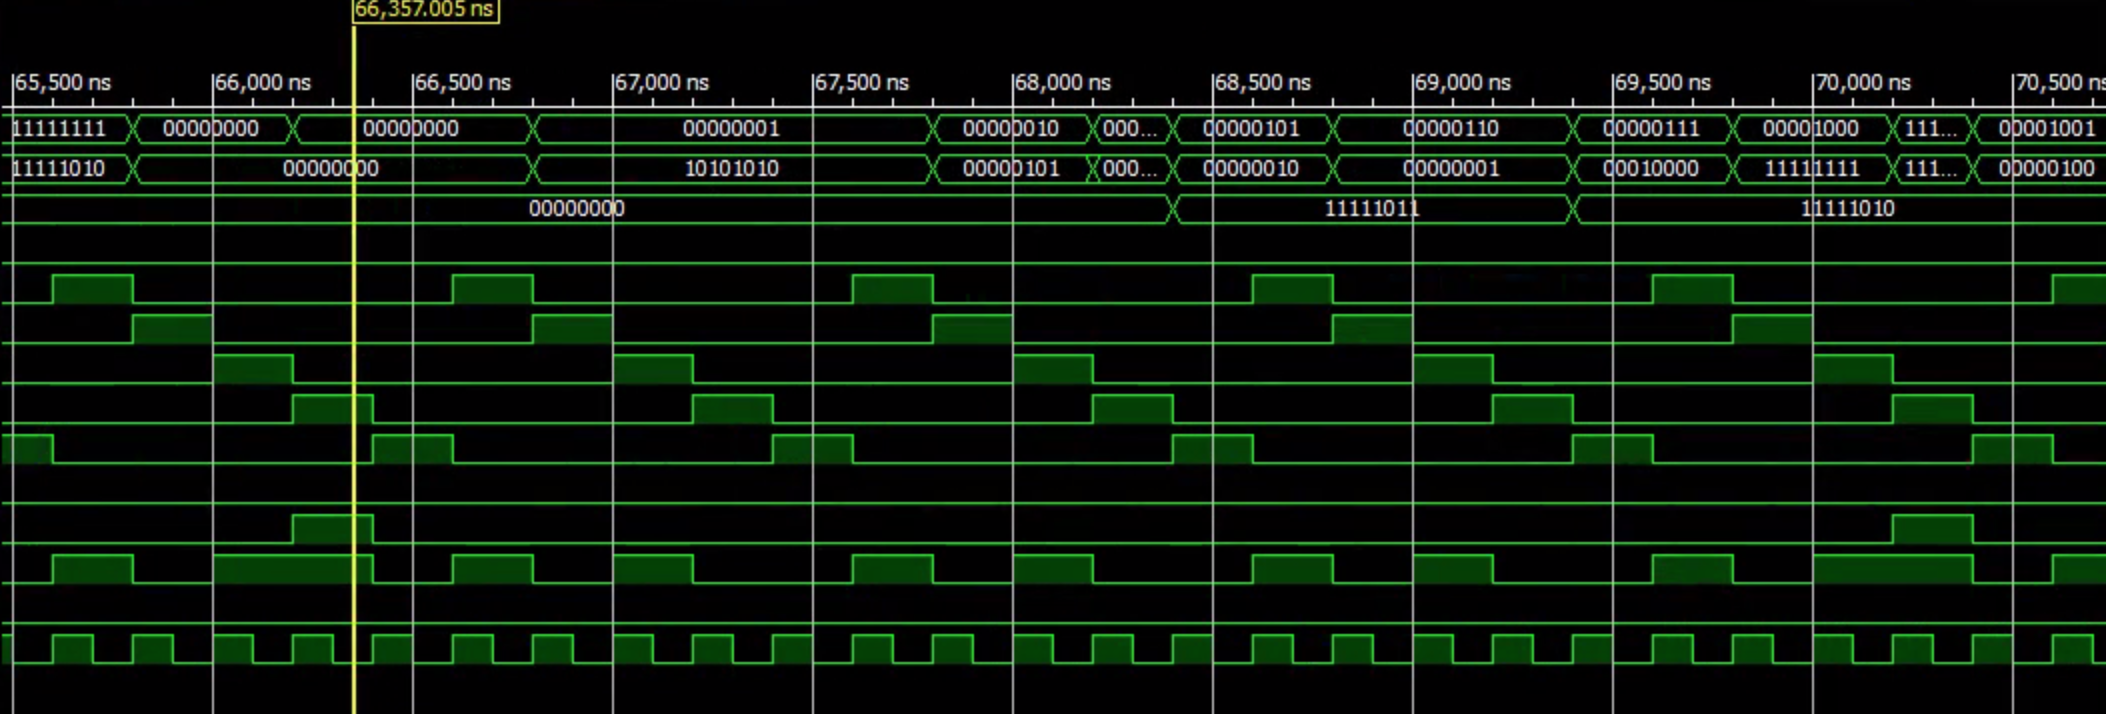
\includegraphics[scale=.4]{tb4.png}\\
	This is the testbench of out Toy\_Overall\_Processor. We wrote the original program from Lab 5 into ROM and you can see that being written to RAM and that the program does not begin running until all of ROM is written to RAM. After that you can see the state changes occuring as they did in the last lab and the program runs as it did in the last lab as well now it is just coming from RAM.
\end{center}

	\newpage
\section{Significance} \vspace{-.7cm} \line(1,0){470}
	\paragraph{} 
		With memory added, we have much more flexibility with what we can input to the Toy Processor. Also, it is 

 \section{Comments/Suggestions}\vspace{-.7cm} \line(1,0){470}
 	\paragraph{} 
 		N.A.
		
\end{document}


